\documentclass{article}
\usepackage[margin=1in]{geometry}
\usepackage{amsmath,amsthm,amssymb}
\usepackage{bbm,enumerate,mathtools}
\usepackage{tikz,pgfplots}
\usepackage{chessboard}
\usepackage[hidelinks]{hyperref}
\usepackage{multicol} % Problem 35
\usepackage{xstring} % Difficulty command
\usetikzlibrary{shapes.geometric}

\newenvironment{question}{\begin{trivlist}\item[\textbf{Question.}]}{\end{trivlist}}
\newenvironment{note}{\begin{trivlist}\item[\textbf{Note.}]}{\end{trivlist}}
\newenvironment{references}{\begin{trivlist}\item[\textbf{References.}]}{\end{trivlist}}
\newenvironment{related}{\begin{trivlist}\item[\textbf{Related.}]\end{trivlist}\begin{enumerate}}{\end{enumerate}}

\newcommand\score[1]{
\pgfmathsetmacro\pgfxa{#1+1}
\tikzstyle{scorestars}=[
  star,
  star points=5,
  star point ratio=2.25,
  draw,
  inner sep=3pt,
  anchor=outer point 5
]
  \begin{tikzpicture}[baseline]
    \draw[opacity=0] (0,-0.5) rectangle (0,0.2); % Workaround for whitespace at the bottom.
    \foreach \i in {1,...,4} {
      \pgfmathparse{(\i<=#1?"yellow":"gray")}
      \edef\starcolor{\pgfmathresult}
      \draw (\i*4.5ex,0) node[name=star\i,scorestars,fill=\starcolor]  {};
    }
  \end{tikzpicture}
}

\newcommand{\difficulty}[1]{%
  \IfEqCase{#1}{%
      {1}{
        
\begin{tikzpicture}[scale=0.7, baseline=0.9mm]%
          \definecolor{slopegreen}{rgb}{0.0, 0.5, 0.0}%
          \fill[slopegreen] (0.5,0.5) circle (0.5);%
        \end{tikzpicture}%
      }%
      {2}{
        
\begin{tikzpicture}[scale=0.7, baseline=0.9mm]%
          \definecolor{slopeblue}{rgb}{0.0, 0.44, 1.00}
          \fill[slopeblue] (0,0) rectangle (1,1);%
        \end{tikzpicture}%
      }%
      {3}{
\begin{tikzpicture}[scale=0.7, baseline=0.9mm]\fill (0,0.5)--(0.5, 0)--(1,0.5)--(0.5,1)--cycle; \end{tikzpicture}}%
      {4}{
\begin{tikzpicture}[scale=0.7, baseline=0.9mm]\fill (0.25,0)--(0,0.5)--(0.25,1)--(0.5,0.5)--cycle; \fill (0.75,0)--(0.5,0.5)--(0.75,1)--(1,0.5)--cycle;\end{tikzpicture}}%
      % you can add more cases here as desired
  }[\PackageError{difficulty}{Undefined difficulty level: #1}{}]%
}%
\newcommand{\rating}[2]{\difficulty{#1}\\\score{#2}\\}


\begin{document}
\rating{4}{3}
The Erd\H{o}s distinct distance problem asks for the number of distinct
distances determined by $n$ points in the Euclidean plane.

\begin{figure}[ht!]
  \centering
  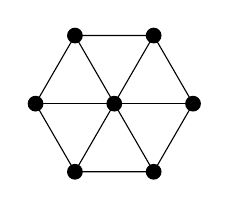
\begin{tikzpicture}
    \fill (0, 0) circle (0.1);
    \fill (1, 0) circle (0.1);
    \fill (3/2, {1.73/2}) circle (0.1);
    \fill (1/2, {1.73/2}) circle (0.1);
    \fill (1, {1.73}) circle (0.1);
    \fill (0, {1.73}) circle (0.1);
    \fill (-1/2, {1.73/2}) circle (0.1);
    \draw (0,0)--(1,0)--(3/2, 1.73/2)--(1,1.73)--(0,1.73)--(-1/2,1.73/2)--cycle;
    \draw (0,0)--(1,1.73);
    \draw (1,0)--(0,1.73);
    \draw (-1/2,1.73/2)--(3/2,1.73/2);
  \end{tikzpicture}
  \hspace{1cm}
  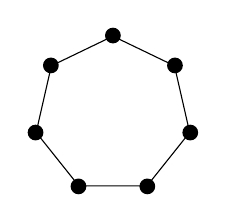
\begin{tikzpicture}
    \node[draw,minimum size=2cm,regular polygon,regular polygon sides=7] (a) {};
    % draw a black dot in each vertex
    \foreach \x in {1,2,...,7}
      \fill (a.corner \x) circle (0.1);
  \end{tikzpicture}
  \\~\\
  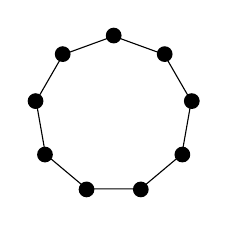
\begin{tikzpicture}
    \node[draw,minimum size=2cm,regular polygon,regular polygon sides=9] (a) {};
    % draw a black dot in each vertex
    \foreach \x in {1,2,...,9}
      \fill (a.corner \x) circle (0.1);
  \end{tikzpicture}
  \hspace{1cm}
  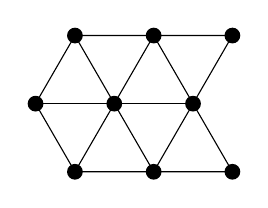
\begin{tikzpicture}
    \fill (0, 0) circle (0.1);
    \fill (1, 0) circle (0.1);
    \fill (2, 0) circle (0.1);
    \fill (3/2, {1.73/2}) circle (0.1);
    \fill (1/2, {1.73/2}) circle (0.1);
    \fill (2, {1.73}) circle (0.1);
    \fill (1, {1.73}) circle (0.1);
    \fill (0, {1.73}) circle (0.1);
    \fill (-1/2, {1.73/2}) circle (0.1);
    \draw (0,0)--(1,0)--(3/2, 1.73/2)--(1,1.73)--(0,1.73)--(-1/2,1.73/2)--cycle;
    \draw (0,0)--(1,1.73)--(2,1.73)--(3/2,1.73/2)--(2,0)--(1,0)--(0,1.73);
    \draw (-1/2,1.73/2)--(3/2,1.73/2);
  \end{tikzpicture}
  \caption{
    Sets with $3$ and $4$ distinct distances on $7$ and $9$ vertices
    respectively. There are no larger sets with an equal or smaller number of
    vertices.
  }
\end{figure}
\begin{question}
  If $n$ points are constrained to the grid $\mathbb Z^2$, what is the minimal
  number of distinct distances?
\end{question}

\begin{related}
  \item How many such figures?
  \item What if the figures are constrained to some subset of $\mathbb Z^2$, e.g. $[n]\times[n]$?
  \item What about on other grids (triangular, hexagonal, etc)?
  \item Can this be meaningfully done on more exotic topologies, e.g. $Z_n^2$?
  \item What about $\mathbb Z^n$ for $n > 2$? What is the asymptotic behavior?
  \item What if distance is measured via $d_1$, $d_3$, or $d_\infty$?
\end{related}

\begin{references}
  \item Problem 34.
  \item \url{https://oeis.org/A186704}: Erd\H{o}s distinct distance problem.
\end{references}

\end{document}
